% Created 2021-02-19 ven. 11:49
% Intended LaTeX compiler: pdflatex
\documentclass[10pt]{iopart}

\expandafter\let\csname equation*\endcsname\relax
\expandafter\let\csname endequation*\endcsname\relax
\usepackage{capt-of, subcaption}
\usepackage[colorlinks=true, allcolors=blue]{hyperref}
\usepackage{amsmath, amssymb, amsfonts, cases, bm}
\usepackage{algorithmic, graphicx, textcomp}
\usepackage{xcolor, import}
\usepackage[USenglish, english]{babel}
\usepackage{siunitx}
\usepackage{tikz}
\usetikzlibrary{shapes.misc,arrows,arrows.meta}
\usepackage[square,comma,sort&compress,numbers]{natbib}
\renewcommand{\bibsection}{\section*{References}}
\hypersetup{
 pdfauthor={Thomas Dehaeze},
 pdftitle={},
 pdfkeywords={},
 pdfsubject={},
 pdfcreator={Emacs 27.1 (Org mode 9.5)}, 
 pdflang={English}}
\begin{document}

\title{Active damping of rotating platforms using integral force feedback}
\author{Thomas Dehaeze$^{1,3}$ and Christophe Collette$^{1,2}$}
\address{$^1$ Precision Mechatronics Laboratory, University of Liege, Belgium}
\address{$^2$ BEAMS Department, Free University of Brussels, Belgium}
\address{$^3$ European Synchrotron Radiation Facility, Grenoble, France}
\ead{tdehaeze@uliege.be}

\begin{abstract}
This paper investigates the use of Integral Force Feedback (IFF) for the active damping of rotating mechanical systems.
Guaranteed stability, typical benefit of IFF, is lost as soon as the system is rotating due to gyroscopic effects.
To overcome this issue, two modifications of the classical IFF control scheme are proposed.
The first consists of slightly modifying the control law while the second consists of adding springs in parallel with the force sensors.
Conditions for stability and optimal parameters are derived.
The results reveal that, despite their different implementations, both modified IFF control scheme have almost identical damping authority on the suspension modes.
\end{abstract}

\vspace{2pc}
\noindent{\it Keywords}: Active Damping, IFF

\submitto{{\it Engineering Research Express\/}}
\maketitle
% Two Columns output
\ioptwocol

\section{Introduction}
\label{sec:org1def047}
\label{sec:introduction}
There is an increasing need to reduce the undesirable vibration of sensitive equipment in many different fields such as in aerospace industry~\cite{hanieh03_activ_stewar,hauge04_sensor_contr_space_based_six,souleille18_concep_activ_mount_space_applic}, semi conductor industry~\cite{yoshioka01_activ_microv_isolat_system_hi}, microscopy~\cite{lan08_activ_vibrat_isolat_long_range,fleming15_low_order_dampin_track_contr}, gravitational wave detectors~\cite{matichard15_seism_isolat_advan_ligo} and particles accelerators~\cite{collette10_activ_quadr_stabil_futur_linear_partic_collid,dehaeze18_sampl_stabil_for_tomog_exper}.

A common method to reduce vibration is to mount the sensitive equipment on a suspended platform which attenuates the vibrations above the frequency of the suspension modes~\cite{reilly06_critic,poel10_explor_activ_hard_mount_vibrat}. \par
In order to further decrease the residual vibrations, active damping can be used for reducing the magnification of the response in the vicinity of the resonances~\cite{collette11_review_activ_vibrat_isolat_strat}.

Many active damping techniques have been developed over the years such as Positive Position Feedback (PPF)~\cite{lin06_distur_atten_precis_hexap_point,fanson90_posit_posit_feedb_contr_large_space_struc}, Integral Force Feedback (IFF)~\cite{preumont91_activ} and Direct Velocity Feedback (DVF)~\cite{karnopp74_vibrat_contr_using_semi_activ_force_gener,serrand00_multic_feedb_contr_isolat_base_excit_vibrat,preumont02_force_feedb_versus_accel_feedb}. \par
In~\cite{preumont92_activ_dampin_by_local_force}, the IFF control scheme has been proposed, where a force sensor, a force actuator and an integral controller are used to directly augment the damping of a mechanical system.
When the force sensor is collocated with the actuator, the open-loop transfer function has alternating poles and zeros which facilitate to guarantee the stability of the closed loop system~\cite{preumont02_force_feedb_versus_accel_feedb}.
It was latter shown that this property holds for multiple collated actuator/sensor pairs~\cite{preumont08_trans_zeros_struc_contr_with}. \par
The main advantages of IFF over other active damping techniques are the guaranteed stability even in presence of flexible dynamics, good performances and robustness properties~\cite{preumont02_force_feedb_versus_accel_feedb}. \par
Several improvements of the classical IFF have been proposed, such as adding a feed-through term to increase the achievable damping~\cite{teo15_optim_integ_force_feedb_activ_vibrat_contr} or adding an high pass filter to recover the loss of compliance at low frequency~\cite{chesne16_enhan_dampin_flexib_struc_using_force_feedb}.
Recently, an \(\mathcal{H}_\infty\) optimization criterion has been used to derive optimal gains for the IFF controller~\cite{zhao19_optim_integ_force_feedb_contr}. \par
However, when the platform is rotating, gyroscopic effects alter the system dynamics and IFF cannot be applied as is.
The purpose of this paper is to study how the IFF strategy can be adapted to deal with these gyroscopic effects. \par
The paper is structured as follows.
Section~\ref{sec:dynamics} presents a simple model of a rotating suspended platform that will be used throughout this study.
Section~\ref{sec:iff} explains how the unconditional stability of IFF is lost due to gyroscopic effects induced by the rotation.
Section~\ref{sec:iff_hpf} suggests a simple modification of the control law such that damping can be added to the suspension modes in a robust way.
Section~\ref{sec:iff_kp} proposes to add springs in parallel with the force sensors to regain the unconditional stability of IFF.
Section~\ref{sec:comparison} compares both proposed modifications to the classical IFF in terms of damping authority and closed-loop system behavior.

\section{Dynamics of Rotating Platforms}
\label{sec:org414e8cb}
\label{sec:dynamics}
In order to study how the rotation affects the use of IFF, a model of a suspended platform on top of a rotating stage is used.
Figure~\ref{fig:system} represents a schematic of the model which is the simplest in which gyroscopic forces can be studied.

\begin{figure}[htbp]
\centering
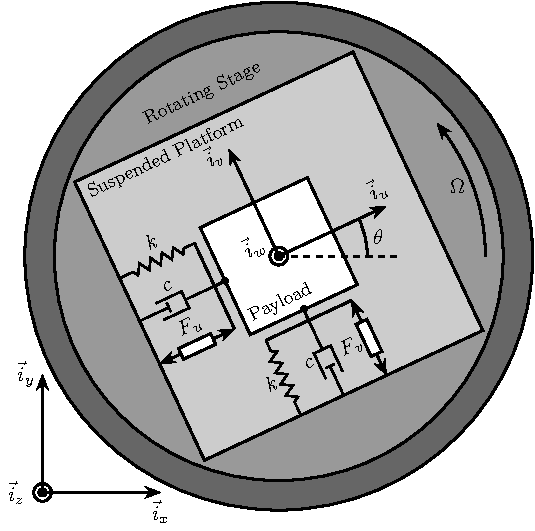
\includegraphics[scale=1,scale=0.9]{figs/fig01.pdf}
\caption{\label{fig:system}Schematic of the studied system}
\end{figure}

The rotating stage is supposed to be ideal, meaning it induces a perfect rotation \(\theta(t) = \Omega t\) where \(\Omega\) is the rotational speed in \(\si{\radian\per\s}\).

The suspended platform consists of two orthogonal actuators each represented by three elements in parallel: a spring with a stiffness \(k\) in \(\si{\newton\per\meter}\), a dashpot with a damping coefficient \(c\) in \(\si{\newton\per(\meter\per\second)^{-1}}\) and an ideal force source \(F_u, F_v\).
A payload with a mass \(m\) in \(\si{\kilo\gram}\), representing the sensitive equipment, is mounted on the (rotating) suspended platform.

Two reference frames are used: an inertial frame \((\vec{i}_x, \vec{i}_y, \vec{i}_z)\) and a uniform rotating frame \((\vec{i}_u, \vec{i}_v, \vec{i}_w)\) rigidly fixed on top of the rotating stage with \(\vec{i}_w\) aligned with the rotation axis.
The position of the payload is represented by \((d_u, d_v, 0)\) expressed in the rotating frame.

\par
To obtain the equations of motion for the system represented in Figure~\ref{fig:system}, the Lagrangian equations are used:
\begin{equation}
\label{eq:lagrangian_equations}
  \frac{d}{dt} \left( \frac{\partial L}{\partial \dot{q}_i} \right) + \frac{\partial D}{\partial \dot{q}_i} - \frac{\partial L}{\partial q_i} = Q_i
\end{equation}
with \(L = T - V\) the Lagrangian, \(T\) the kinetic coenergy, \(V\) the potential energy, \(D\) the dissipation function, and \(Q_i\) the generalized force associated with the generalized variable \(\begin{bmatrix}q_1 & q_2\end{bmatrix} = \begin{bmatrix}d_u & d_v\end{bmatrix}\).
The equation of motion corresponding to the constant rotation along \(\vec{i}_w\) is disregarded as this motion is considered to be imposed by the rotation stage.
\begin{equation}
\label{eq:energy_functions_lagrange}
  \begin{aligned}
    T &= \frac{1}{2} m \left( ( \dot{d}_u - \Omega d_v )^2 + ( \dot{d}_v + \Omega d_u )^2 \right), \\
    V &= \frac{1}{2} k \big( {d_u}^2 + {d_v}^2 \big), \ Q_1 = F_u, \\
    D &= \frac{1}{2} c \big( \dot{d}_u{}^2 + \dot{d}_v{}^2 \big), \ Q_2 = F_v
  \end{aligned}
\end{equation}

Substituting Eq.~\eqref{eq:energy_functions_lagrange} into Eq.~\eqref{eq:lagrangian_equations} for both generalized coordinates gives two coupled differential equations~\eqref{eq:eom_coupled_1} and~\eqref{eq:eom_coupled_2}.
\begin{subequations}
\label{eq:eom_coupled}
  \begin{align}
    m \ddot{d}_u + c \dot{d}_u + ( k - m \Omega^2 ) d_u &= F_u + 2 m \Omega \dot{d}_v \label{eq:eom_coupled_1} \\
    m \ddot{d}_v + c \dot{d}_v + ( k \underbrace{-\,m \Omega^2}_{\text{Centrif.}} ) d_v &= F_v \underbrace{-\,2 m \Omega \dot{d}_u}_{\text{Coriolis}} \label{eq:eom_coupled_2}
  \end{align}
\end{subequations}

The uniform rotation of the system induces two gyroscopic effects as shown in Eq.~\eqref{eq:eom_coupled}:
\begin{itemize}
\item Centrifugal forces: that can been seen as an added negative stiffness \(- m \Omega^2\) along \(\vec{i}_u\) and \(\vec{i}_v\)
\item Coriolis Forces: that adds coupling between the two orthogonal directions.
\end{itemize}

One can verify that without rotation (\(\Omega = 0\)) the system becomes equivalent to two uncoupled one degree of freedom mass-spring-damper systems.

\par
To study the dynamics of the system, the differential equations of motions~\eqref{eq:eom_coupled} are converted into the Laplace domain and the \(2 \times 2\) transfer function matrix \(\mathbf{G}_d\) from \(\begin{bmatrix}F_u & F_v\end{bmatrix}\) to \(\begin{bmatrix}d_u & d_v\end{bmatrix}\) in Eq.~\eqref{eq:Gd_mimo_tf} is obtained.
Its elements are shown in Eq.~\eqref{eq:Gd_indiv_el}.

\begin{equation}
\label{eq:Gd_mimo_tf}
  \begin{bmatrix} d_u \\ d_v \end{bmatrix} = \mathbf{G}_d \begin{bmatrix} F_u \\ F_v \end{bmatrix}
\end{equation}


\begin{subequations}
\label{eq:Gd_indiv_el}
\begin{align}
  & \mathbf{G}_{d}(1,1) = \mathbf{G}_{d}(2,2) = \dots \nonumber \\
  & \quad {\frac{ms^2 + cs + k - m \Omega^2}{\left( m s^2 + cs + k - m \Omega^2 \right)^2 + \left( 2 m \Omega s \right)^2}} \\
  & \mathbf{G}_{d}(1,2) = -\mathbf{G}_{d}(1,2) = \dots \nonumber \\
  & \quad {\frac{2 m \Omega s}{\left( m s^2 + cs + k - m \Omega^2 \right)^2 + \left( 2 m \Omega s \right)^2}}
\end{align}
\end{subequations}

To simplify the analysis, the undamped natural frequency \(\omega_0\) and the damping ratio \(\xi\) are used as in Eq.~\eqref{eq:xi_and_omega}.
\begin{equation}
\label{eq:xi_and_omega}
  \omega_0 = \sqrt{\frac{k}{m}} \text{ in } \si{\radian\per\second}, \quad \xi = \frac{c}{2 \sqrt{k m}}
\end{equation}

The elements of transfer function matrix \(\mathbf{G}_d\) are now describe by Eq.~\eqref{eq:Gd_w0_xi_k}.
\begin{subequations}
\label{eq:Gd_w0_xi_k}
  \begin{align}
    \mathbf{G}_{d}(1,1) &= {\scriptstyle \frac{\frac{1}{k} \left( \frac{s^2}{{\omega_0}^2} + 2 \xi \frac{s}{\omega_0} + 1 - \frac{{\Omega}^2}{{\omega_0}^2} \right)}{\left( \frac{s^2}{{\omega_0}^2} + 2 \xi \frac{s}{\omega_0} + 1 - \frac{{\Omega}^2}{{\omega_0}^2} \right)^2 + \left( 2 \frac{\Omega}{\omega_0} \frac{s}{\omega_0} \right)^2}}  \\
    \mathbf{G}_{d}(1,2) &= {\scriptstyle \frac{\frac{1}{k} \left( 2 \frac{\Omega}{\omega_0} \frac{s}{\omega_0} \right)}{\left( \frac{s^2}{{\omega_0}^2} + 2 \xi \frac{s}{\omega_0} + 1 - \frac{{\Omega}^2}{{\omega_0}^2} \right)^2 + \left( 2 \frac{\Omega}{\omega_0} \frac{s}{\omega_0} \right)^2}}
  \end{align}
\end{subequations}

For all further numerical analysis in this study, we consider \(\omega_0 = \SI{1}{\radian\per\second}\), \(k = \SI{1}{\newton\per\meter}\) and \(\xi = 0.025 = \SI{2.5}{\percent}\).
Even though no system with such parameters will be encountered in practice, conclusions can be drawn relative to these parameters such that they can be generalized to any other set of parameters.

\par
The poles of \(\mathbf{G}_d\) are the complex solutions \(p\) of Eq.~\eqref{eq:poles}.

\begin{equation}
\label{eq:poles}
  \left( \frac{p^2}{{\omega_0}^2} + 2 \xi \frac{p}{\omega_0} + 1 - \frac{{\Omega}^2}{{\omega_0}^2} \right)^2 + \left( 2 \frac{\Omega}{\omega_0} \frac{p}{\omega_0} \right)^2 = 0
\end{equation}

Supposing small damping (\(\xi \ll 1\)), two pairs of complex conjugate poles are obtained as shown in Eq.~\eqref{eq:pole_values}.

\begin{subequations}
\label{eq:pole_values}
  \begin{align}
    p_{+} &= - \xi \omega_0 \left( 1 + \frac{\Omega}{\omega_0} \right) \pm j \omega_0 \left( 1 + \frac{\Omega}{\omega_0} \right) \\
    p_{-} &= - \xi \omega_0 \left( 1 - \frac{\Omega}{\omega_0} \right) \pm j \omega_0 \left( 1 - \frac{\Omega}{\omega_0} \right)
  \end{align}
\end{subequations}

The real and complex parts of these two pairs of complex conjugate poles are represented in Figure~\ref{fig:campbell_diagram} as a function of the rotational speed \(\Omega\).
As the rotational speed increases, \(p_{+}\) goes to higher frequencies and \(p_{-}\) goes to lower frequencies.
The system becomes unstable for \(\Omega > \omega_0\) as the real part of \(p_{-}\) is positive.
Physically, the negative stiffness term \(-m\Omega^2\) induced by centrifugal forces exceeds the spring stiffness \(k\).

In the rest of this study, rotational speeds smaller than the undamped natural frequency of the system are assumed (\(\Omega < \omega_0\)).

\begin{figure}[htbp]
\begin{subfigure}[c]{0.48\linewidth}
\centering
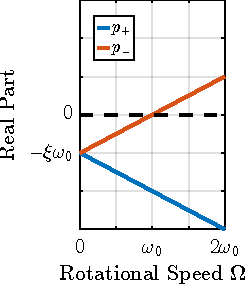
\includegraphics[scale=1]{figs/fig02a.pdf}
\caption{\label{fig:campbell_diagram_real} Real Part}
\end{subfigure}
\hfill
\begin{subfigure}[c]{0.48\linewidth}
\centering
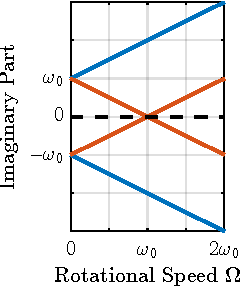
\includegraphics[scale=1]{figs/fig02b.pdf}
\caption{\label{fig:campbell_diagram_imag} Imaginary Part}
\end{subfigure}
\hfill
\caption{\label{fig:campbell_diagram}Campbell diagram : Evolution of the complex and real parts of the system's poles as a function of the rotational speed \(\Omega\)}
\centering
\end{figure}

Looking at the transfer function matrix \(\mathbf{G}_d\) in Eq.~\eqref{eq:Gd_w0_xi_k}, one can see that the two diagonal (direct) terms are equal and that the two off-diagonal (coupling) terms are opposite.
The bode plot of these two terms are shown in Figure~\ref{fig:plant_compare_rotating_speed} for several rotational speeds \(\Omega\).
These plots confirm the expected behavior: the frequency of the two pairs of complex conjugate poles are further separated as \(\Omega\) increases.
For \(\Omega > \omega_0\), the low frequency pair of complex conjugate poles \(p_{-}\) becomes unstable.

\begin{figure}[htbp]
\begin{subfigure}[c]{0.48\linewidth}
\centering
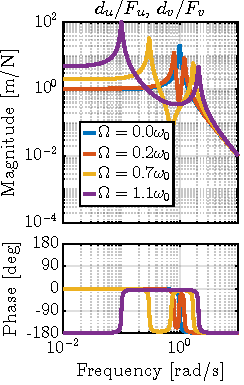
\includegraphics[scale=1]{figs/fig03a.pdf}
\caption{\label{fig:plant_compare_rotating_speed_direct} Direct Terms}
\end{subfigure}
\hfill
\begin{subfigure}[c]{0.48\linewidth}
\centering
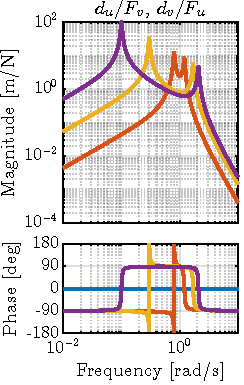
\includegraphics[scale=1]{figs/fig03b.pdf}
\caption{\label{fig:plant_compare_rotating_speed_coupling} Coupling Terms}
\end{subfigure}
\hfill
\caption{\label{fig:plant_compare_rotating_speed}Bode plots for \(\mathbf{G}_d\) for several rotational speed \(\Omega\)}
\centering
\end{figure}

\section{Decentralized Integral Force Feedback}
\label{sec:orgdc87c6d}
\label{sec:iff}
In order to apply IFF to the rotating system, force sensors are added in series with the two actuators (Figure~\ref{fig:system_iff}).
As this study focuses on decentralized control, two identical controllers \(K_F\) are used to feedback each of the sensed force to its associated actuator and no attempt is made to counteract the interactions in the system.
The control diagram is schematically shown in Figure~\ref{fig:control_diagram_iff}.

\begin{figure}[htbp]
\centering
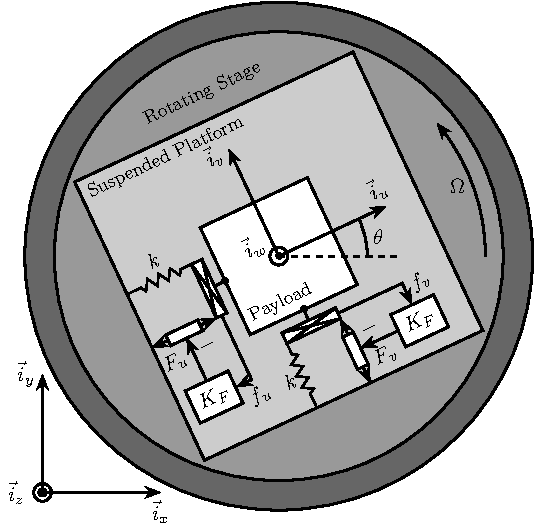
\includegraphics[scale=1,scale=0.9]{figs/fig04.pdf}
\caption{\label{fig:system_iff}System with added force sensor in series with the actuators and with a decentralized IFF architecture}
\end{figure}

\begin{figure}[htbp]
\centering
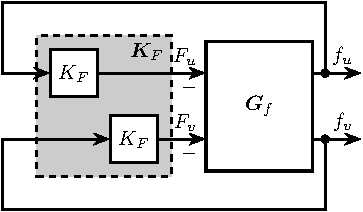
\includegraphics[scale=1,scale=1]{figs/fig05.pdf}
\caption{\label{fig:control_diagram_iff}Control diagram for decentralized IFF}
\end{figure}

\par
The forces \(\begin{bmatrix}f_u & f_v\end{bmatrix}\) measured by the two force sensors represented in Figure~\ref{fig:system_iff} are described by Eq.~\eqref{eq:measured_force}.
\begin{equation}
\label{eq:measured_force}
  \begin{bmatrix} f_{u} \\ f_{v} \end{bmatrix} =
  \begin{bmatrix} F_u \\ F_v \end{bmatrix} - (c s + k)
  \begin{bmatrix} d_u \\ d_v \end{bmatrix}
\end{equation}

The transfer function matrix \(\mathbf{G}_{f}\) from actuator forces to measured forces in Eq.~\eqref{eq:Gf_mimo_tf} can be obtained by inserting Eq.~\eqref{eq:Gd_w0_xi_k} into Eq.~\eqref{eq:measured_force}.
Its elements are shown in Eq.~\eqref{eq:Gf_indiv_el}.

\begin{equation}
\label{eq:Gf_mimo_tf}
  \begin{bmatrix} f_{u} \\ f_{v} \end{bmatrix} = \mathbf{G}_{f} \begin{bmatrix} F_u \\ F_v \end{bmatrix}
\end{equation}

\begin{subequations}
\label{eq:Gf_indiv_el}
\label{eq:Gf}
  \begin{align}
    & \mathbf{G}_{f}(1,1) = \mathbf{G}_{f}(2,2) = \dots \nonumber \\
    & \quad {\scriptstyle \frac{\left( \frac{s^2}{{\omega_0}^2} - \frac{\Omega^2}{{\omega_0}^2} \right) \left( \frac{s^2}{{\omega_0}^2} + 2 \xi \frac{s}{\omega_0} + 1 - \frac{{\Omega}^2}{{\omega_0}^2} \right) + \left( 2 \frac{\Omega}{\omega_0} \frac{s}{\omega_0} \right)^2}{\left( \frac{s^2}{{\omega_0}^2} + 2 \xi \frac{s}{\omega_0} + 1 - \frac{{\Omega}^2}{{\omega_0}^2} \right)^2 + \left( 2 \frac{\Omega}{\omega_0} \frac{s}{\omega_0} \right)^2} } \label{eq:Gf_diag_tf} \\
    & \mathbf{G}_{f}(1,2) = -\mathbf{G}_{f}(2,1) = \dots \nonumber \\
    & \quad {\scriptstyle \frac{- \left( 2 \xi \frac{s}{\omega_0} + 1 \right) \left( 2 \frac{\Omega}{\omega_0} \frac{s}{\omega_0} \right)}{\left( \frac{s^2}{{\omega_0}^2} + 2 \xi \frac{s}{\omega_0} + 1 - \frac{{\Omega}^2}{{\omega_0}^2} \right)^2 + \left( 2 \frac{\Omega}{\omega_0} \frac{s}{\omega_0} \right)^2} } \label{eq:Gf_off_diag_tf}
  \end{align}
\end{subequations}

The zeros of the diagonal terms of \(\mathbf{G}_f\) in Eq.~\eqref{eq:Gf_diag_tf} are computed, and neglecting the damping for simplicity, two complex conjugated poles \(z_{c}\) are obtained in Eq.~\eqref{eq:iff_zero_cc}, and two real zeros \(z_{r}\) in Eq.~\eqref{eq:iff_zero_real}.
\begin{subequations}
  \begin{align}
    z_c &= \pm j \omega_0 \sqrt{\frac{1}{2} \sqrt{8 \frac{\Omega^2}{{\omega_0}^2} + 1} + \frac{\Omega^2}{{\omega_0}^2} + \frac{1}{2} } \label{eq:iff_zero_cc} \\
    z_r &= \pm   \omega_0 \sqrt{\frac{1}{2} \sqrt{8 \frac{\Omega^2}{{\omega_0}^2} + 1} - \frac{\Omega^2}{{\omega_0}^2} - \frac{1}{2} } \label{eq:iff_zero_real}
  \end{align}
\end{subequations}

It is interesting to see that the frequency of the pair of complex conjugate zeros \(z_c\) in Eq.~\eqref{eq:iff_zero_cc} always lies between the frequency of the two pairs of complex conjugate poles \(p_{-}\) and \(p_{+}\) in Eq.~\eqref{eq:pole_values}.

For non-null rotational speeds, the two real zeros \(z_r\) in Eq.~\eqref{eq:iff_zero_real} induce a non-minimum phase behavior.
This can be seen in the Bode plot of the diagonal terms (Figure~\ref{fig:plant_iff_compare_rotating_speed}) where the low frequency gain is no longer zero while the phase stays at \(\SI{180}{\degree}\).

The low frequency gain of \(\mathbf{G}_f\) increases with the rotational speed \(\Omega\) as shown in Eq.~\eqref{eq:low_freq_gain_iff_plan}.
\begin{equation}
\label{eq:low_freq_gain_iff_plan}
  \lim_{\omega \to 0} \left| \mathbf{G}_f (j\omega) \right| = \begin{bmatrix}
  \frac{\Omega^2}{{\omega_0}^2 - \Omega^2} & 0 \\
  0  & \frac{\Omega^2}{{\omega_0}^2 - \Omega^2}
\end{bmatrix}
\end{equation}

This can be explained as follows: a constant force \(F_u\) induces a small displacement of the mass \(d_u = \frac{F_u}{k - m\Omega^2}\), which increases the centrifugal force \(m\Omega^2d_u = \frac{\Omega^2}{{\omega_0}^2 - \Omega^2} F_u\) which is then measured by the force sensors.

\begin{figure}[htbp]
\centering
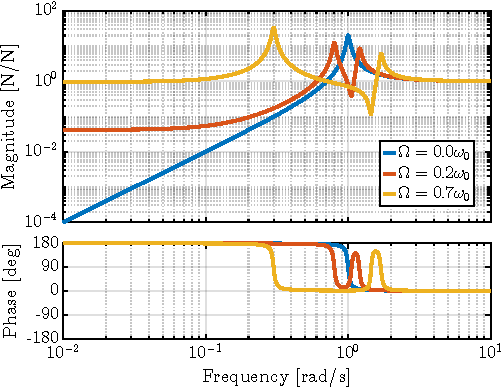
\includegraphics[scale=1,scale=0.95]{figs/fig06.pdf}
\caption{\label{fig:plant_iff_compare_rotating_speed}Bode plot of the dynamics from a force actuator to its collocated force sensor (\(f_u/F_u\), \(f_v/F_v\)) for several rotational speeds \(\Omega\)}
\end{figure}

\par
\label{sec:iff_pure_int}
The two IFF controllers \(K_{F}\) consist of a pure integrator as shown in Eq.~\eqref{eq:Kf_pure_int} where \(g\) is a scalar representing the gain of the controller.
\begin{equation}
\label{eq:Kf_pure_int}
\begin{aligned}
  \mathbf{K}_{F}(s) &= \begin{bmatrix} K_{F}(s) & 0 \\ 0 & K_{F}(s) \end{bmatrix} \\
  K_{F}(s) &= g \cdot \frac{1}{s}
\end{aligned}
\end{equation}

In order to see how the IFF controller affects the poles of the closed loop system, a Root Locus plot (Figure~\ref{fig:root_locus_pure_iff}) is constructed as follows: the poles of the closed-loop system are drawn in the complex plane as the controller gain \(g\) varies from \(0\) to \(\infty\) for the two controllers \(K_{F}\) simultaneously.
As explained in~\cite{preumont08_trans_zeros_struc_contr_with,skogestad07_multiv_feedb_contr}, the closed-loop poles start at the open-loop poles (shown by \(\tikz[baseline=-0.6ex] \node[cross out, draw=black, minimum size=1ex, line width=2pt, inner sep=0pt, outer sep=0pt] at (0, 0){};\)) for \(g = 0\) and coincide with the transmission zeros (shown by \(\tikz[baseline=-0.6ex] \draw[line width=2pt, inner sep=0pt, outer sep=0pt] (0,0) circle[radius=3pt];\)) as \(g \to \infty\).
The direction of increasing gain is indicated by arrows \(\tikz[baseline=-0.6ex] \draw[-{Stealth[round]},line width=2pt] (0,0) -- (0.3,0);\).

\begin{figure}[htbp]
\centering
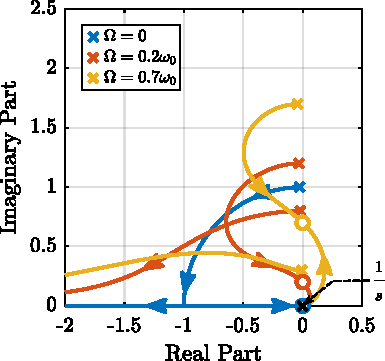
\includegraphics[scale=1,scale=1]{figs/fig07.pdf}
\caption{\label{fig:root_locus_pure_iff}Root Locus: Evolution of the closed-loop poles with increasing controller gains \(g\)}
\end{figure}

Whereas collocated IFF is usually associated with unconditional stability~\cite{preumont91_activ}, this property is lost due to gyroscopic effects as soon as the rotational speed in non-null.
This can be seen in the Root Locus plot (Figure~\ref{fig:root_locus_pure_iff}) where poles corresponding to the controller are bound to the right half plane implying closed-loop system instability.

Physically, this can be explained like so: at low frequency, the loop gain is very large due to the pure integrator in \(K_{F}\) and the finite gain of the plant (Figure~\ref{fig:plant_iff_compare_rotating_speed}).
The control system is thus canceling the spring forces which makes the suspended platform no able to hold the payload against centrifugal forces, hence the instability.

In order to apply decentralized IFF to rotating platforms, two solutions are proposed to deal with this instability problem.
The first one consists of slightly modifying the control law (Section~\ref{sec:iff_hpf}) while the second one consists of adding springs in parallel with the force sensors (Section~\ref{sec:iff_kp}).

\section{Integral Force Feedback with High Pass Filter}
\label{sec:orgdb88ec7}
\label{sec:iff_hpf}
As was explained in the previous section, the instability comes in part from the high gain at low frequency caused by the pure integrators.

In order to limit the low frequency controller gain, an High Pass Filter (HPF) can be added to the controller as shown in Eq.~\eqref{eq:IFF_LHF}.

\begin{equation}
\label{eq:IFF_LHF}
  K_{F}(s) = g \cdot \frac{1}{s} \cdot \underbrace{\frac{s/\omega_i}{1 + s/\omega_i}}_{\text{HPF}} = g \cdot \frac{1}{s + \omega_i}
\end{equation}

This is equivalent as to slightly shifting the controller pole to the left along the real axis.

This modification of the IFF controller is typically done to avoid saturation associated with the pure integrator~\cite{preumont91_activ,marneffe07_activ_passiv_vibrat_isolat_dampin_shunt_trans}.
This is however not the case in this study as it will become clear in the next section.

\par
The loop gains, \(K_F(s)\) times the direct dynamics \(f_u/F_u\), with and without the added HPF are shown in Figure~\ref{fig:loop_gain_modified_iff}.
The effect of the added HPF limits the low frequency gain as expected.

The Root Locus plots for the decentralized IFF with and without the HPF are displayed in Figure~\ref{fig:root_locus_modified_iff}.
With the added HPF, the poles of the closed loop system are shown to be stable up to some value of the gain \(g_\text{max}\) in Eq.~\eqref{eq:gmax_iff_hpf}.

\begin{equation}
\label{eq:gmax_iff_hpf}
  g_{\text{max}} = \omega_i \left( \frac{{\omega_0}^2}{\Omega^2} - 1 \right)
\end{equation}

It is interesting to note that \(g_{\text{max}}\) also corresponds to the controller gain at which the low frequency loop gain (Figure~\ref{fig:loop_gain_modified_iff}) reaches one.

\begin{figure}[htbp]
\centering
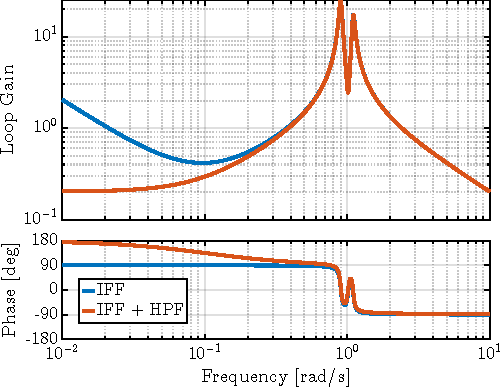
\includegraphics[scale=1,scale=0.95]{figs/fig08.pdf}
\caption{\label{fig:loop_gain_modified_iff}Modification of the loop gain with the added HFP, \(g = 2\), \(\omega_i = 0.1 \omega_0\) and \(\Omega = 0.1 \omega_0\)}
\end{figure}

\begin{figure}[htbp]
\centering
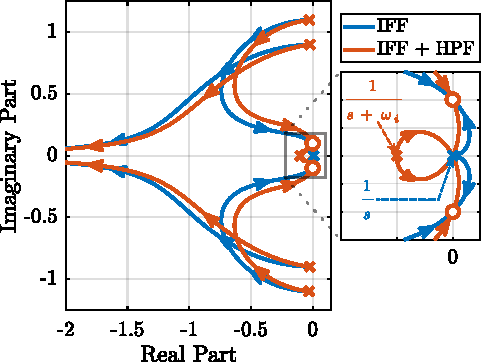
\includegraphics[scale=1,scale=1]{figs/fig09.pdf}
\caption{\label{fig:root_locus_modified_iff}Modification of the Root Locus with the added HPF, \(\omega_i = 0.1 \omega_0\) and \(\Omega = 0.1 \omega_0\)}
\end{figure}

\par
Two parameters can be tuned for the modified controller in Eq.~\eqref{eq:IFF_LHF}: the gain \(g\) and the pole's location \(\omega_i\).
The optimal values of \(\omega_i\) and \(g\) are here considered as the values for which the damping of all the closed-loop poles are simultaneously maximized.

In order to visualize how \(\omega_i\) does affect the attainable damping, the Root Locus plots for several \(\omega_i\) are displayed in Figure~\ref{fig:root_locus_wi_modified_iff}.
It is shown that even though small \(\omega_i\) seem to allow more damping to be added to the suspension modes, the control gain \(g\) may be limited to small values due to Eq.~\eqref{eq:gmax_iff_hpf}.

\begin{figure}[htbp]
\centering
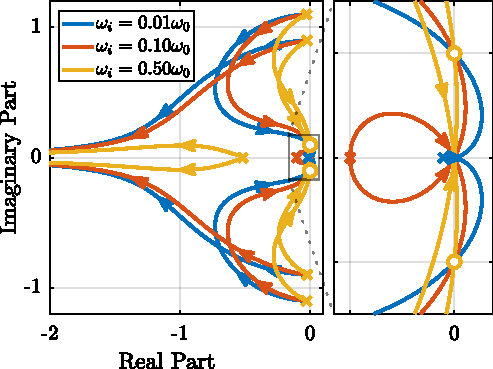
\includegraphics[scale=1,scale=0.95]{figs/fig10.pdf}
\caption{\label{fig:root_locus_wi_modified_iff}Root Locus for several HPF cut-off frequencies \(\omega_i\), \(\Omega = 0.1 \omega_0\)}
\end{figure}

In order to study this trade off, the attainable closed-loop damping ratio \(\xi_{\text{cl}}\) is computed as a function of \(\omega_i/\omega_0\).
The gain \(g_{\text{opt}}\) at which this maximum damping is obtained is also displayed and compared with the gain \(g_{\text{max}}\) at which the system becomes unstable (Figure~\ref{fig:mod_iff_damping_wi}).

\begin{figure}[htbp]
\centering
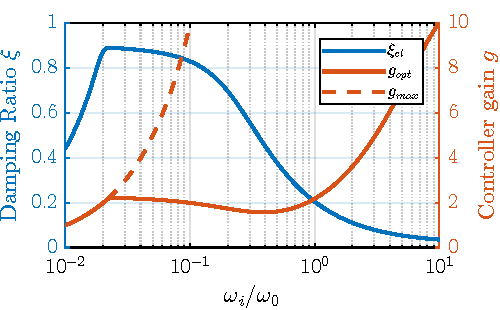
\includegraphics[scale=1,scale=0.95]{figs/fig11.pdf}
\caption{\label{fig:mod_iff_damping_wi}Attainable damping ratio \(\xi_\text{cl}\) as a function of \(\omega_i/\omega_0\). Corresponding control gain \(g_\text{opt}\) and \(g_\text{max}\) are also shown}
\end{figure}

Three regions can be observed:
\begin{itemize}
\item \(\omega_i/\omega_0 < 0.02\): the added damping is limited by the maximum allowed control gain \(g_{\text{max}}\)
\item \(0.02 < \omega_i/\omega_0 < 0.2\): the attainable damping ratio is maximized and is reached for \(g \approx 2\)
\item \(0.2 < \omega_i/\omega_0\): the added damping decreases as \(\omega_i/\omega_0\) increases.
\end{itemize}

\section{Integral Force Feedback with Parallel Springs}
\label{sec:org19946d1}
\label{sec:iff_kp}
In this section additional springs in parallel with the force sensors are added to counteract the negative stiffness induced by the gyroscopic effects.
Such springs are schematically shown in Figure~\ref{fig:system_parallel_springs} where \(k_a\) is the stiffness of the actuator and \(k_p\) the stiffness in parallel with the actuator and force sensor.

Amplified piezoelectric stack actuators can be used for such purpose where a part of the piezoelectric stack is used as an actuator while the rest is used as a force sensor~\cite{souleille18_concep_activ_mount_space_applic}.
The parallel stiffness \(k_p\) then corresponds to the mechanical amplification structure.

\begin{figure}[htbp]
\centering
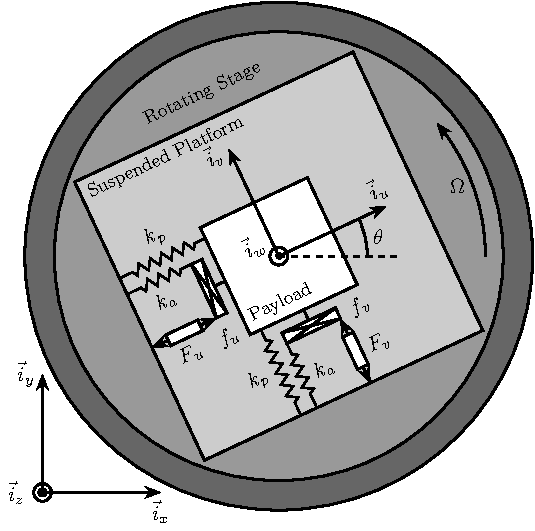
\includegraphics[scale=1,scale=0.9]{figs/fig12.pdf}
\caption{\label{fig:system_parallel_springs}Studied system with additional springs in parallel with the actuators and force sensors}
\end{figure}

\par
The forces measured by the two force sensors represented in Figure~\ref{fig:system_parallel_springs} are described by Eq.~\eqref{eq:measured_force_kp}.

\begin{equation}
\label{eq:measured_force_kp}
  \begin{bmatrix} f_{u} \\ f_{v} \end{bmatrix} =
  \begin{bmatrix} F_u \\ F_v \end{bmatrix} - (c s + k_a)
  \begin{bmatrix} d_u \\ d_v \end{bmatrix}
\end{equation}

In order to keep the overall stiffness \(k = k_a + k_p\) constant, thus not modifying the open-loop poles as \(k_p\) is changed, a scalar parameter \(\alpha\) (\(0 \le \alpha < 1\)) is defined to describe the fraction of the total stiffness in parallel with the actuator and force sensor as in Eq.~\eqref{eq:kp_alpha}.

\begin{equation}
\label{eq:kp_alpha}
  k_p = \alpha k, \quad k_a = (1 - \alpha) k
\end{equation}

After the equations of motion derived and transformed in the Laplace domain, the transfer function matrix \(\mathbf{G}_k\) in Eq.~\eqref{eq:Gk_mimo_tf} is computed.
Its elements are shown in Eq.~\eqref{eq:Gk_diag} and~\eqref{eq:Gk_off_diag}.

\begin{equation}
\label{eq:Gk_mimo_tf}
  \begin{bmatrix} f_u \\ f_v \end{bmatrix} =
  \mathbf{G}_k
  \begin{bmatrix} F_u \\ F_v \end{bmatrix}
\end{equation}

\begin{subequations}
\label{eq:Gk}
\begin{align}
& \mathbf{G}_{k}(1,1) = \mathbf{G}_{k}(2,2) = \dots \nonumber \\
& \quad {\scriptstyle \frac{\big( \frac{s^2}{{\omega_0}^2} - \frac{\Omega^2}{{\omega_0}^2} + \alpha \big) \big( \frac{s^2}{{\omega_0}^2} + 2 \xi \frac{s}{\omega_0} + 1 - \frac{{\Omega}^2}{{\omega_0}^2} \big) + \big( 2 \frac{\Omega}{\omega_0} \frac{s}{\omega_0} \big)^2}{\big( \frac{s^2}{{\omega_0}^2} + 2 \xi \frac{s}{\omega_0} + 1 - \frac{{\Omega}^2}{{\omega_0}^2} \big)^2 + \big( 2 \frac{\Omega}{\omega_0} \frac{s}{\omega_0} \big)^2} } \label{eq:Gk_diag} \\
& \mathbf{G}_{k}(1,2) = -\mathbf{G}_{k}(2,1) = \dots \nonumber \\
& \quad {\scriptscriptstyle \frac{- \left( 2 \xi \frac{s}{\omega_0} + 1 - \alpha \right) \left( 2 \frac{\Omega}{\omega_0} \frac{s}{\omega_0} \right)}{\left( \frac{s^2}{{\omega_0}^2} + 2 \xi \frac{s}{\omega_0} + 1 - \frac{{\Omega}^2}{{\omega_0}^2} \right)^2 + \left( 2 \frac{\Omega}{\omega_0} \frac{s}{\omega_0} \right)^2} } \label{eq:Gk_off_diag}
\end{align}
\end{subequations}

Comparing \(\mathbf{G}_k\) in Eq.~\eqref{eq:Gk} with \(\mathbf{G}_f\) in Eq.~\eqref{eq:Gf} shows that while the poles of the system are kept the same, the zeros of the diagonal terms have changed.
The two real zeros \(z_r\) in Eq.~\eqref{eq:iff_zero_real} that were inducing a non-minimum phase behavior are transformed into two complex conjugate zeros if the condition in Eq.~\eqref{eq:kp_cond_cc_zeros} holds.

\begin{equation}
\label{eq:kp_cond_cc_zeros}
  \alpha > \frac{\Omega^2}{{\omega_0}^2} \quad \Leftrightarrow \quad k_p > m \Omega^2
\end{equation}

Thus, if the added parallel stiffness \(k_p\) is higher than the negative stiffness induced by centrifugal forces \(m \Omega^2\), the dynamics from actuator to its collocated force sensor will show minimum phase behavior.
This is confirmed by the Bode plot in Figure~\ref{fig:plant_iff_kp}.

Figure~\ref{fig:root_locus_iff_kp} shows the Root Locus plots for \(k_p = 0\), \(k_p < m \Omega^2\) and \(k_p > m \Omega^2\) when \(K_F\) is a pure integrator as in Eq.~\eqref{eq:Kf_pure_int}.
It is shown that if the added stiffness is higher than the maximum negative stiffness, the poles of the closed-loop system are bounded on the (stable) left half-plane, and hence the unconditional stability of IFF is recovered.

\begin{figure}[htbp]
\centering
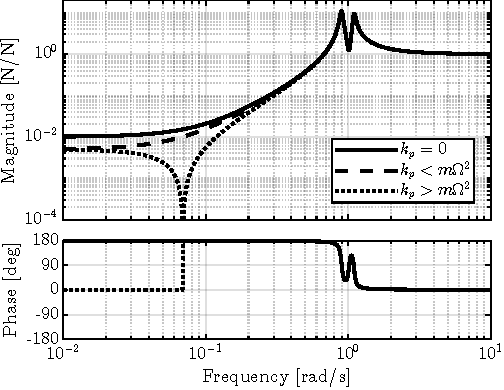
\includegraphics[scale=1,scale=0.95]{figs/fig13.pdf}
\caption{\label{fig:plant_iff_kp}Bode plot of \(G_{k}(1,1) = f_u/F_u\) without parallel spring, with parallel spring stiffness \(k_p < m \Omega^2\) and \(k_p > m \Omega^2\), \(\Omega = 0.1 \omega_0\)}
\end{figure}

\begin{figure}[htbp]
\centering
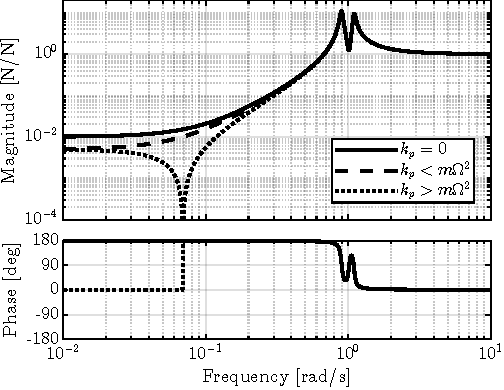
\includegraphics[scale=1,scale=0.95]{figs/fig14.pdf}
\caption{\label{fig:root_locus_iff_kp}Root Locus for IFF without parallel spring, with parallel spring stiffness \(k_p < m \Omega^2\) and \(k_p > m \Omega^2\), \(\Omega = 0.1 \omega_0\)}
\end{figure}

\par
Even though the parallel stiffness \(k_p\) has no impact on the open-loop poles (as the overall stiffness \(k\) is kept constant), it has a large impact on the transmission zeros.
Moreover, as the attainable damping is generally proportional to the distance between poles and zeros~\cite{preumont18_vibrat_contr_activ_struc_fourt_edition}, the parallel stiffness \(k_p\) is foreseen to have a large impact on the attainable damping.

To study this effect, Root Locus plots for several parallel stiffnesses \(k_p > m \Omega^2\) are shown in Figure~\ref{fig:root_locus_iff_kps}.
The frequencies of the transmission zeros of the system are increasing with an increase of the parallel stiffness \(k_p\) and the associated attainable damping is reduced.
Therefore, even though the parallel stiffness \(k_p\) should be larger than \(m \Omega^2\) for stability reasons, it should not be taken too large as this would limit the attainable damping.

This is confirmed by the Figure~\ref{fig:opt_damp_alpha} where the attainable closed-loop damping ratio \(\xi_{\text{cl}}\) and the associated optimal control gain \(g_\text{opt}\) are computed as a function of \(\alpha\).

\begin{figure}[htbp]
\centering
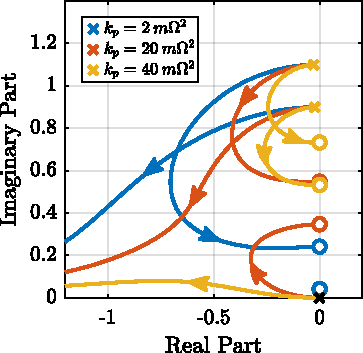
\includegraphics[scale=1,scale=1]{figs/fig15.pdf}
\caption{\label{fig:root_locus_iff_kps}Comparison of the Root Locus plots for three parallel stiffnessses \(k_p\)}
\end{figure}


\begin{figure}[htbp]
\centering
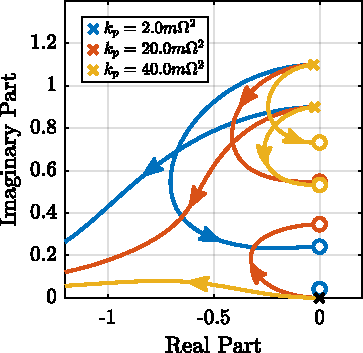
\includegraphics[scale=1,scale=0.95]{figs/fig16.pdf}
\caption{\label{fig:opt_damp_alpha}Optimal damping ratio \(\xi_\text{opt}\) and the corresponding optimal gain \(g_\text{opt}\) as a function of \(\alpha\)}
\end{figure}

\section{Comparison and Discussion}
\label{sec:org3688d53}
\label{sec:comparison}
In order to overcome the instability issue of the classical IFF strategy when applied to rotating platforms, two modifications of IFF have been proposed in Sections~\ref{sec:iff_hpf} and~\ref{sec:iff_kp}.
These two methods are now compared in terms of added damping, closed-loop compliance and transmissibility.

For the following comparisons, the cut-off frequency for the HPF is set to \(\omega_i = 0.1 \omega_0\) and the stiffness of the parallel springs is set to \(k_p = 5 m \Omega^2\) (corresponding to \(\alpha = 0.05\)).
These values are chosen based on the discussion about optimal parameters.

\par
Figure~\ref{fig:comp_root_locus} shows the Root Locus plots for the two proposed IFF modifications.
While the two pairs of complex conjugate open-loop poles are identical for both techniques, the transmission zeros are not.
This means that the closed-loop behavior of both systems will differ when large control gains are used.

One can observe that the closed loop poles corresponding to the system with added springs (in red) are bounded to the left half plane implying unconditional stability.
This is not the case for the system where the controller is augmented with an HPF (in blue).

It is interesting to note that the maximum added damping is very similar for both techniques and is reached for the same control gain \(g_\text{opt} \approx 2 \omega_0\).

\begin{figure}[htbp]
\centering
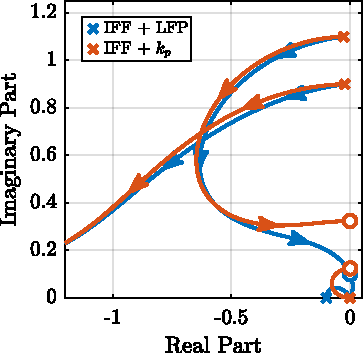
\includegraphics[scale=1,scale=1]{figs/fig17.pdf}
\caption{\label{fig:comp_root_locus}Root Locus for the two proposed modifications of decentralized IFF, \(\Omega = 0.1 \omega_0\)}
\end{figure}

\par
The two proposed techniques are now compared in terms of closed-loop transmissibility and compliance.

The transmissibility is here defined as the transfer function from a displacement of the rotating stage along \(\vec{i}_x\) to the displacement of the payload along the same direction.
It is used to characterize how much vibration is transmitted through the suspended platform to the payload.

The compliance describes the displacement response of the payload to external forces applied to it.
This is a useful metric when disturbances are directly applied to the payload.
It is here defined as the transfer function from external forces applied on the payload along \(\vec{i}_x\) to the displacement of the payload along the same direction.

The two techniques are also compared with passive damping (Figure~\ref{fig:system}) where the damping coefficient \(c\) is tuned to critically damp the resonance when the rotating speed is null as shown in Eq.~\eqref{eq:critical_damp}.
\begin{equation}
\label{eq:critical_damp}
  c_\text{crit} = 2 \sqrt{k m}
\end{equation}

Very similar results are obtained for the two proposed IFF modifications in terms of transmissibility (Figure~\ref{fig:comp_transmissibility}) and compliance (Figure~\ref{fig:comp_compliance}).
It is also confirmed that these two techniques can significantly damp the suspension modes.

\begin{figure}[htbp]
\centering
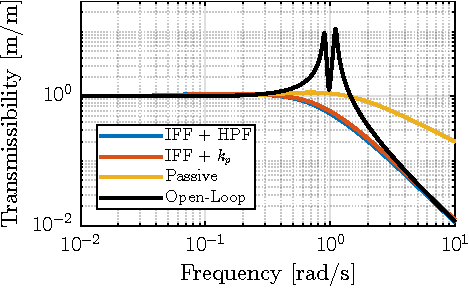
\includegraphics[scale=1,scale=1]{figs/fig18.pdf}
\caption{\label{fig:comp_transmissibility}Comparison of the two proposed active damping techniques - transmissibility}
\end{figure}


\begin{figure}[htbp]
\centering
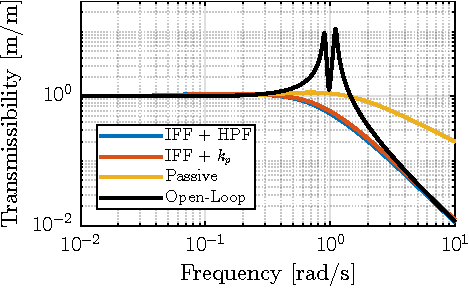
\includegraphics[scale=1,scale=1]{figs/fig19.pdf}
\caption{\label{fig:comp_compliance}Comparison of the two proposed active damping techniques - compliance}
\end{figure}

On can see in Figure~\ref{fig:comp_transmissibility} that the problem of the degradation of the transmissibility at high frequency when using passive damping techniques is overcome by the use of IFF.

The addition of the HPF or the use of the parallel stiffness also permits to limit the degradation of the compliance as compared with classical IFF (Figure~\ref{fig:comp_compliance}).

\section{Conclusion}
\label{sec:org2f060ad}
\label{sec:conclusion}

Due to gyroscopic effects, decentralized IFF with pure integrators was shown to be unstable when applied to rotating platforms.
Two modifications of the classical IFF control have been proposed to overcome this issue.

The first modification concerns the controller and consists of adding an high pass filter to the pure integrators.
This is equivalent as to moving the controller pole to the left along the real axis.
This allows the closed loop system to be stable up to some value of the controller gain.

The second proposed modification concerns the mechanical system.
Additional springs are added in parallel with the actuators and force sensors.
It was shown that if the stiffness \(k_p\) of the additional springs is larger than the negative stiffness \(m \Omega^2\) induced by centrifugal forces, the classical decentralized IFF regains its unconditional stability property.

While having very different implementations, both proposed modifications are very similar when it comes to the attainable damping and the obtained closed loop system behavior.

Future work will focus on the experimental validation of the proposed IFF modifications.

\section*{Data Availability}
\label{sec:org6c5e786}
Matlab~\cite{matlab20} was used for this study.
The source code is available under a MIT License and archived in Zenodo~\cite{dehaeze20_activ_dampin_rotat_posit_platf}.

\section*{Acknowledgments}
\label{sec:org2c37487}
This research benefited from a FRIA grant (grant number: FC 31597) from the French Community of Belgium.
This paper is based on a paper previously presented at the ISMA conference~\cite{dehaeze20_activ_dampin_rotat_platf_integ_force_feedb}.

\bibliographystyle{iopart-num}
\bibliography{ref}
\end{document}
